%\documentclass{emulateapj}
\documentclass[12pt,preprint]{aastex}

%\documentclass{aastex}

\usepackage{verbatim}

\slugcomment{Last revision \today}

% A comment block

%\newcommand{\comment}[1]{}

% For color
\newcommand{\mpname}[1]{#1_color.eps}
\newcommand{\clraitoff}{red}
\newcommand{\lumblack}{(black)}
\newcommand{\lumblue}{(blue)}
\newcommand{\lumred}{(red)}
\newcommand{\vdisred}{(red-dashed curve)}
\newcommand{\vdisblue}{(blue-solid curve)}

% For bw
%\newcommand{\mpname}[1]{#1.eps}
%\newcommand{\clraitoff}{}
%\newcommand{\lumblack}{}
%\newcommand{\lumblue}{}
%\newcommand{\lumred}{}
%\newcommand{\vdisred}{(dashed curve)}
%\newcommand{\vdisblue}{(solid curve)}

\newcommand{\umag}{$u$}
\newcommand{\gmag}{$g$}
\newcommand{\rmag}{$r$}
\newcommand{\imag}{$i$}
\newcommand{\zmag}{$z$}
\newcommand{\gmr}{$g-r$}



\newcommand{\gammat}{$\gamma_T$}
\newcommand{\gammacross}{$\gamma_\times$}
\newcommand{\deltasig}{$\Delta \Sigma$}
\newcommand{\deltaplus}{$\Delta \Sigma_+$}
\newcommand{\deltacross}{$\Delta \Sigma_\times$}
\newcommand{\deltarho}{$\Delta \rho$}
\newcommand{\movr}{$M(<r)$}
\newcommand{\sigmacrit}{$\Sigma_{crit}$}

\newcommand{\photoz}{photo-z}
\newcommand{\photozs}{photo-zs}

\newcommand{\tlum}{$L^{tot}$}
\newcommand{\tngal}{$N_{gal}^{tot}$}

\newcommand{\lstarlim}{$0.4 L_*$}
\newcommand{\lvir}{$L_{200}$}
\newcommand{\lvirtot}{$L^{tot}_{200}$}
\newcommand{\mvir}{$M_{200}$}
\newcommand{\nvir}{$N_{200}$}
\newcommand{\rvirgal}{$r_{200}^{gals}$}
\newcommand{\rvirmass}{$r_{200}^{mass}$}

\newcommand{\deltamtol}{$\Delta M/\Delta L$}
\newcommand{\deltam}{$\Delta M$}
\newcommand{\deltal}{$\Delta L$}

\newcommand{\deltamvir}{$\Delta M_{200}$}
\newcommand{\deltalvir}{$\Delta L_{200}$}

\newcommand{\mtolmax}{$(\Delta M/\Delta L)_{22\mathrm{Mpc}}$}
\newcommand{\mtolasym}{$(\Delta M/\Delta L)_{asym}$}
\newcommand{\mtolvir}{$(\Delta M/\Delta L)_{200}$}
\newcommand{\bmtol}{$b^2_{M/L}$}
\newcommand{\bmtolinv}{$b^{-2}_{M/L}$}

\newcommand{\ngal}{$N_{gal}$}
\newcommand{\maxbcg}{MaxBCG}
\newcommand{\numNgalBins}{12}
\newcommand{\numLumBins}{16}

\newcommand{\tngalAperture}{2$h^{-1}$ Mpc}

\newcommand{\photo}{\texttt{PHOTO}}
\newcommand{\astrop}{\texttt{ASTRO}}
\newcommand{\mt}{\texttt{MT}}
\newcommand{\spectro}{\texttt{SPECTRO}}
\newcommand{\spectroone}{\texttt{SPECTRO1d}}
\newcommand{\spectrotwo}{\texttt{SPECTRO2d}}
\newcommand{\target}{\texttt{TARGET}}

\newcommand{\lenszmax}{0.3}
\newcommand{\lenszmin}{0.05}
\newcommand{\zmean}{0.25}

\newcommand{\photoversion}{\texttt{v5\_4}}

%\def\eone{e$_1$}
%\def\etwo{e$_2$}
\newcommand{\etan}{e$_+$}
\newcommand{\erad}{e$_\times$}
\newcommand{\eclass}{\texttt{ECLASS}}
\newcommand{\eclasscut}{-0.06}
\newcommand{\gmrcut}{0.7}

\newcommand{\hrs}{$^{\mathrm h}$}
\newcommand{\minutes}{$^{\mathrm m}$}

\newcommand{\ugriz}{$u, g, r, i, z$}
\newcommand{\polarization}{polarization}

\newcommand{\wgm}{$w_{gm}$}
\newcommand{\wgg}{$w_{gg}^p$}
\newcommand{\wmm}{$w_{mm}$}
\newcommand{\xigg}{$\xi_{gg}$}
\newcommand{\ximm}{$\xi_{mm}$}
\newcommand{\xigm}{$\xi_{gm}$}

\newcommand{\numspec}{127,001}
\newcommand{\numspecvlim}{10,277}
\newcommand{\numrand}{1,270,010}
\newcommand{\numspectot}{278,192}
\newcommand{\numvdis}{49,024}
%\newcommand{\numsource}{10,259,949}
% hirata: 
\newcommand{\nummask}{1,815,043}
\newcommand{\numTenMpc}{132,473}
\newcommand{\numThirtyMpc}{101,221}
\newcommand{\numsource}{27,912,891}

\newcommand{\numpairsTenMpc}{2,670,898,177}
\newcommand{\altnumpairsTenMpc}{2.7 billion}
\newcommand{\numpairsThirtyMpc}{14,818,082,122}
\newcommand{\altnumpairsThirtyMpc}{14.8 billion}



\newcommand{\xirmax}{$\xi_{gm}(R_{max})$}

\def \epssmall {0.7}

\newcommand{\magcut}{24.1}

\shortauthors{Sheldon}
\shorttitle{Scaling Predictions}

\begin{document}

\title{Predictions of the Measurement Precision in Future Lensing Surveys}


\author{ Erin S. Sheldon,\altaffilmark{1} }

\altaffiltext{1}{Department of Physics, New York University, 4 Washington Place, New York, NY 10003.}

\begin{abstract} 

In this document I calculate the predicted sensitivity for DES.  I extend the
previous predictions to sensitivity as a function of source redshift for use in
cosmic shear type studies, as well as sensitivity as a function of lens
redshift for cross-correlation lensing studies.  The framework presented is
general, but I apply it directly to DES predictions.

\end{abstract}

\newpage
\tableofcontents


\section{Introduction} \label{sec:intro}

The noise for a given lensing measurement depends basically on the number of
sources, the variance in intrinsic shapes for that source poplulation, and the
noise on individual shape measurements. The signal depends on the the mass of
the lensing matter and the redshift distributions of lenses and sources.  Most
calculations of the predicted signal-to-noise ratio (S/N) simply take these
numbers at face value, which is adequate in many situations. 

The most important factor left out of standard calculations is redshift
dependent shear noise. Fainter source galaxies are noisier and are thus
downweighted, as are smaller galaxies for which the PSF smearing is more
significant. Both of these properties, faintness and smallness, are correlated
with redshift. 

This weighting effectively alters the source redshift distribution.  Although
this is a secondary consideration relative to determining the actual redshift
distribution, it is important for interpreting, or predicting, very precise
measurements. It is also important for cross-correlation lensing when the lens
redshift is high enough that a large fraction of the sources get little weight.

In this paper I will show formulas that explicitly account for this weighting
and apply them in predicting sensitivity in the Dark Energy Survey (DES).  I'll
discuss other sources of noise that aren't easily modeled or predicted and
discuss how to account for these by normalizing to existing measurements.

\section{Signal and Noise} \label{sec:SignalAndNoise}

I'll discuss two types of measurements, the simpler cosmic shear measurements
and the more complex cross-correlation measurements.  Cosmic shear is simpler
because it is an angular correlation function which has no explicit noise
weighting that depends on redshift.

\subsection{Cosmic Shear}

All cosmic shear measurements are essentially shear-shear correlation
functions.  The correlation between pairs at a given separation is calculated,
which contains a convolution of the source galaxy redshift distribution with
itself.  In interpreting the signal, one estimates the redshift distribution of
the sources and models the redshift distribution for the intervening matter and
the correlation function of that intervening matter.  To make predictions for a
given survey one follows essentially the same approach, modeling the redshift
distributions and underlying cosmology.  This measurement involves integrals
over the source redshift distribution such as (leaving out some terms for
clarity):
\begin{equation}
S(r) = \eta A \int dz_L \int dz_S w(z_S) \chi(z_L,z_S) P(z_S),
\end{equation} 
where $\eta$ is the number density of sources per unit area of sky, $A$ is the
area of the survey, $\chi(z_L)$ is a geometrical factor, and $w(z_S)$ is an
inverse shear variance weight factor, which depends implicitly on source
redshift because higher redshift galaxies are less precisely measured, as
discussed in the introduction.   

The usual approach is to account for this weighting simply by modifying the
number density to be an effective density $\eta_{eff}$.  This is equivalent to
assuming the weight is not a function of source redshift, that all sources get
the same weight, thus reducing the effective number density by some factor.
The recovered signal when modeled, or the the predicted signal for a future
survey, will be incorrect because the assumed $w(z_S)$ is not included in the
integral. The weight generally will reduce the signal because lower redshift
sources get sheared less than higher redshift sources.


\subsection{Cross-correlation, or Object Lensing} \label{sec:ccweight}

Consider a measurement of the mean mass of set of lenses, e.g. clusters in a
richness range, or galaxies of a given luminosity. Let the lenses have redshift
distribution $N(z_L)$ and probability distribution of mass profiles
$P(M(R)|z_L)$. Let the sources have angular density $\eta$ and redshift
probability distribution $P(z_S)$.  Let the weight for a source-lens pair be
$w(z_L, z_S)$ as discussed in the introduction.  Finally assume, for
simplicity, that the mass is the observable (which it is not). Then the mean
mass is given by
\begin{equation} \label{eq:meanmass}
\langle M \rangle = 
\int dz_L N(z_L) 
\int dM P(M(R)|z_L) 
\int_0^{R200(M)} dR \frac{2 \pi R}{D^2(z_L)}
\int dz_S \eta P(z_S) w(z_L, z_S) M(z_L, R).
\end{equation}
The variance is essentially one over this formula with the weight
squared and the mass replaced by $(M-\langle M \rangle)^2$.

Note, the actual observable is the shear $\gamma$, which is converted
into the redshift-independent quantity \deltasig:
\begin{equation}
\Delta\Sigma \equiv \gamma \times \Sigma_{crit}(z_L,z_S)
\end{equation}
and that quantity is averaged. The results for many sources are averaged for
each lens, and the results for many lenses are averaged to get the mean
\deltasig.  

As with cosmic shear, part of the weight factor is an inverse variance weight
that depends implicitly on source redshift.  For cross-correlations there is an
additional explicit dependence on lens and source redshift through
$\Sigma_{crit}$:
\begin{equation} \label{eq:wofzl}
    w(z_L, z_S) = 
    \frac
    {1}
    {(\sigma_{SN}^2 + \sigma_{i}^2) \Sigma^2_{crit}(z_L, z_S)}
\end{equation}
Note when the lens redshift is high, so that a large fraction of the sources
are downweighted or even in front of the lens, the resulting signal to noise is
different than predicted ignoring these redshift dependencies.

\section{Other Sources of Noise}

\subsection{Cosmic Shear}

\subsection{Cross-correlation Lensing}

Additional noise in \deltasig\ comes from a number of sources.  There are
sources of noise that are not easily accounted for, such as added variance from
corrections that must be applied to the \deltasig\ profiles. For example, some
sources are clustered for the lenses and the correction factor must be
calculated from the data.  Also, to extract masses without modeling, the
\deltasig\ radial profile must be inverted, which increases the noise.  

I think it is better for our purposes to account for these sources of noise by
normalizing the result to existing measurements rather than modeling them
directly. In that case, all that matters for the prediction are the redshift
distributions and weight factor $w(z_L, z_S)$.  The redshift range for the
lenses can be made relatively small such that the mass profiles will not vary
significantly in the redshift bin.  Then the mass within r200 is essentially an
overall scaling.

Under these assumptions, the relavent quantity for scaling existing
results to another survey is then
\begin{equation} \label{eq:factor}
S = 
\eta \int_{z1}^{z2} dz_L N(z_L) 
\int_0^{R200(M)} dR \frac{2 \pi R}{D(z_L)^2}
\int dz_S P(z_S) w(z_L, z_S),
\end{equation}
where I have just dropped factors that do not matter for the relative scaling.
This can be compared, for example, to the existing results if the masses and
profiles are close to the same.

\section{DES Predictions}

The source and lens redshift distributions can be reasonably predicted for a
survey such as DES based on deep redshift surveys.  I will focus on predicting
the shear noise, but will incorporate redshift distributions from other
sourceslater. I currently have simulations based upon the GOODS data from which
I can predict the weight as a function of magnitude given the noise and seeing
properties of a given survey.  When combined with photometric redshifts these
weights can be used to predict lensing.

The effective number density in the proposal was the total integrated over
source redshift:
\begin{equation}
\eta_{eff} = \eta \int dz_S P(z_S) w(z_S).
\end{equation}
This is appropriate for predictions of cosmic shear sensitivity, but in order
to model the result we also need $w(z_S)$.  Also, for cross-correlation lensing
we need to account for additional explicit weights as a function of lens and
source redshift (see \S \ref{sec:ccweight}).  Due to that weighting clusters at
higher redshift will only use the fainter and smaller galaxies.  The S/N for
these measurements will be suppressed compared to the current predictions 
based just on the total $\eta_{eff}$.

\subsection{Predictions for Cosmic Shear}

The mean relative weight as a function of i-band magnitude is shown in Figure
\ref{fig:weight-mag} for a seeing of 0.9''.  The number density and effective
number density as a function of i-band magnitude are shown in figure
\ref{fig:neff-mag}.  Note, the unweighted number density is higher than it
would be in an actual image because the catalogs were derived from HST images;
most of the faint objects would simply not be detected, and they have a
corresponding low weight.

\epsscale{0.5}
\begin{figure}[p]
    \plotone{plots/des5yr-convolved-maxmag30.0-seeing0.90-weight-vs-mag.eps}
    
    \caption{Relative weight as a function of i-band magnitude for seeing of
    0.9''.  The histogram in magnitude is shown as the solid curve.  Note, in
    practice objects will be cut at around i=\magcut. \label{fig:weight-mag}}

\end{figure}

\begin{figure}[p]
    \plotone{plots/des5yr-convolved-maxmag30.0-seeing0.90-density-vs-mag.eps}
    
    \caption{Number density and effective number density as a function of
    i-band magnitude for seeing=0.9'' \label{fig:neff-mag}}

\end{figure}

The effective density, integrated over all magnitudes, is shown in figure
\ref{fig:neff-seeing} as a function of seeing.  

\begin{figure}[p]
    \centering
    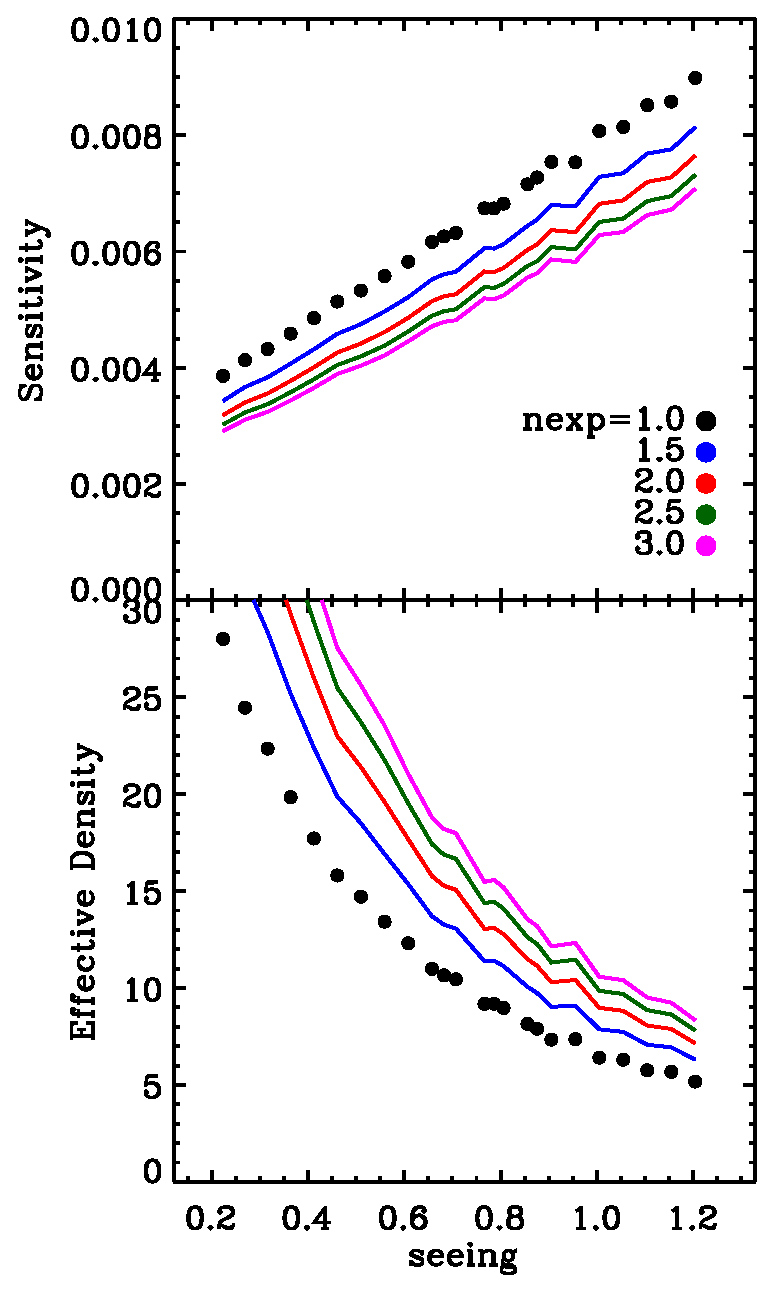
\includegraphics[scale=0.6]{plots/des5yr-convolved-maxmag30.0-neff-vs-seeing.eps}
    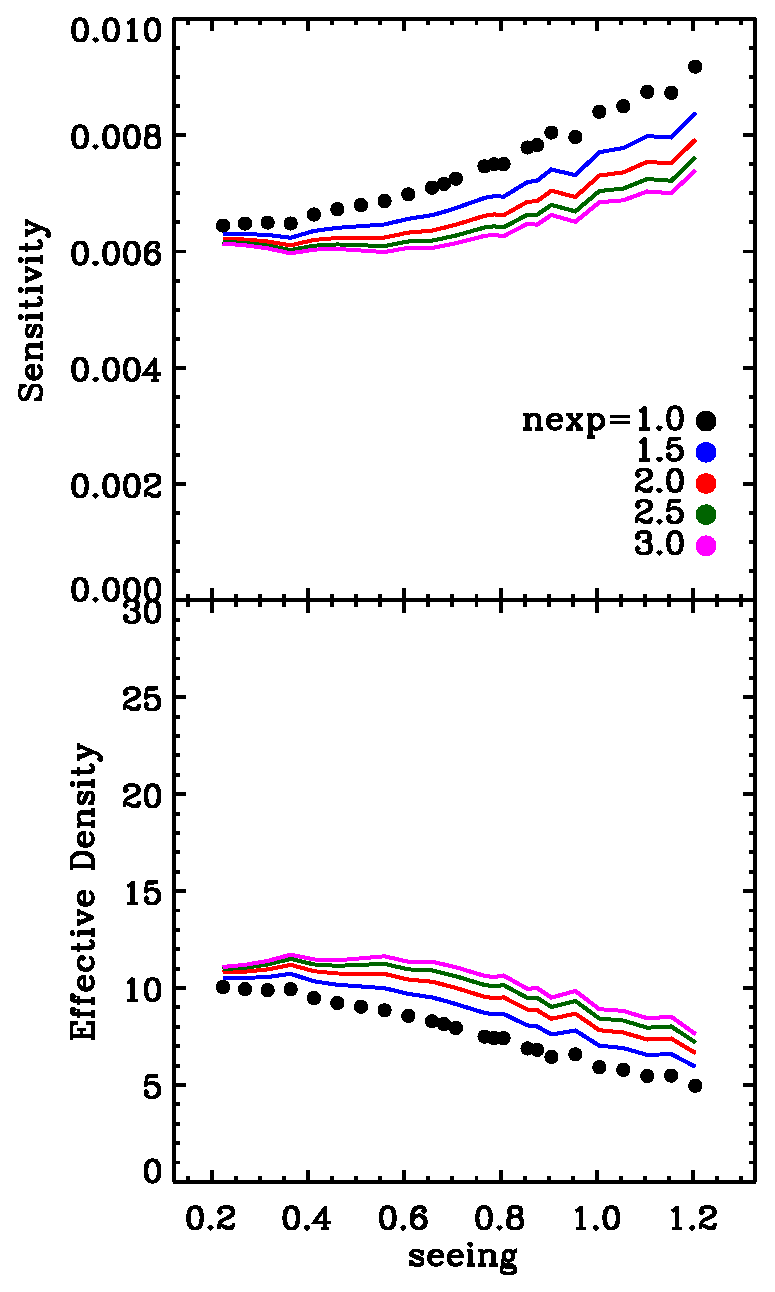
\includegraphics[scale=0.6]{plots/des5yr-convolved-maxmag24.1-neff-vs-seeing.eps}

    \caption{Left Panel: Effective density as a function of seeing with no
explicit magnitude cut.  Points are the des 5yr i-band predictions.  Colored
lines represent additional exposures from other bandpasses, where nexp is the
number of equivalent i-band sensitivity images.  Right panel: Same as the left
panel except with an explicit magnitude cut at i=\magcut. In comparison with
the left panel, this demonstrates the significant extra information at fainter
magnitudes for very good seeing.  The difference for typical seeing (0.9) is
small. \label{fig:neff-seeing} }

\end{figure}


\subsection{Adding Other Filters}

I estimated the expected improvement in the shape measurement error with more
exposures, with an eye to including more bandpasses.  Because the shape noise
is unchanged when using the same objects with more images, the improvement in
sensitivity is limited.  Since there is no plan to coadd different bands, this
is a good assumption.  These curves are shown in the preceding figures
and labeled by the number of effective 5 year i-band sensitivity images.

\subsection{Effective Number Density as Function of Source Redshift}

The effective number density as a function of source redshift can be calculated
form $\eta_{eff}(m_i)$ and an estimate of the redshift distribution in 
magnitude bins $P(z_S|m_i)$.
\begin{equation}
    \eta_{eff}(z_S) = \int dm_i P(z_S|m_i) 
\end{equation}
Haun Lin has provided estimates of $P(z_S|m_i)$ from {\bf need details from
Huan Here}.  These estimates are shown in figure \ref{fig:pzm}.  I interpolated
these curves to a finer grid of magnitudes in the calculationis that follow.

The resulting $\eta_{eff} (z_S)$ for different seeing values, with an explicit
magnitude cut at i=\magcut, are shown in Figure \ref{fig:neff-vs-zs}.

\epsscale{0.7}
\begin{figure}
    \plotone{plots/lfmodel-out-zdist-hdf-IAB-combined-nofz.eps}
    \caption{Estimated $P(z_S | m_i)$ for DES from Huan Lin. {\bf Need details.}
    \label{fig:pzm}}
\end{figure}

\begin{figure}
    \plotone{plots/des5yr-convolved-maxmag24.1-neff-vs-zs.eps}

    \caption{Effective density as a function of source redshift for a range of
seeing values, calculated using the effective density as a function of
magnitude from Figure \ref{fig:weight-mag} and the  $P(z_S | m_i)$ shown in
figure \ref{fig:pzm}. A cut was made at i=\magcut.  \label{fig:neff-vs-zs}}

\end{figure}
\epsscale{1.0}

\subsection{Effective Number Density as Function of Lens Redshift}

In order to calculate $\eta_{eff}(z_L)$, I re-calculated the sensitivity using
the weights shown in Equation \ref{eq:wofzl}.  For the source redshifts, I drew
from the $P(z_S|m_i)$ interpolated to a finer grid of magnitudes.  This Monte
Carlo was repeated 10 times and averaged.  The results are shown in figure
\ref{fig:neff-vs-zl} for an explicit magnitude cut at i=\magcut.

\begin{figure}
    \plotone{plots/des5yr-convolved-maxmag24.1-neff-vs-zl.eps}

    \caption{Effective density as a function of lens redshift for a range of
    seeing values. A cut was made at i=\magcut.  An explicit weighting with
    lens and source redshift is included as described in the text.
    \label{fig:neff-vs-zl}} 
    
\end{figure}


\newpage
\appendix
\section{Appendix: Data}

Two FITS files containing predictions for DES 5yr i-band data are available
from the Wiki.  There is one with an explicit magnitude cut at i=\magcut\ and
one without.  The files have the following structure as seen from an IDL
perspective:
\begin{verbatim}
IDL> help,t30,/str
** Structure <b61498>, 26 tags, length=4832, data length=4828, refs=1:
   SEEING          DOUBLE          0.22360680
   MED_SEEING      DOUBLE          0.24474379
   SHAPENOISE      DOUBLE          0.32000000
   AREA            DOUBLE           61.295800
   RAW_DENSITY     DOUBLE           77.574646
   SHEAR_SENS      DOUBLE        0.0038612918
   NEFF            DOUBLE           28.011993
   SHEAR_SENS_SHONLY
                   DOUBLE        0.0026181055
   NEFF_SHONLY     DOUBLE           60.930533
   SHEAR_SENS3     DOUBLE        0.0030886095
   NEFF3           DOUBLE           43.780755
   MULTI_NEXP      DOUBLE    Array[5]
   MULTI_SENS_FAC  DOUBLE    Array[5]
   MULTI_NEFF_FAC  DOUBLE    Array[5]
   MAG_AUTO        DOUBLE    Array[35]
   MWEIGHT         DOUBLE    Array[35]
   MWEIGHT_ERR     DOUBLE    Array[35]
   MHIST           LONG      Array[35]
   MDENSITY        DOUBLE    Array[35]
   MSHEAR_SENS     DOUBLE    Array[35]
   MNEFF           DOUBLE    Array[35]
   ZS              DOUBLE    Array[25]
   ZSNEFF          DOUBLE    Array[25]
   ZL              DOUBLE    Array[100]
   ZLSENS          DOUBLE    Array[100]
   ZLNEFF          DOUBLE    Array[100]
\end{verbatim}
There is a row in the file for each value of seeing.  Note that in
\texttt{IDL}, long is a 32-bit integer.

The actual median seeing in the images is \texttt{MED\_SEEING}.  The total
effective source density per square arcminute is \texttt{NEFF}.  The
sensitivity in the GOODS images, from which \texttt{NEFF} was derived, is
\texttt{SHEAR\_SENS}.   The magnitude-dependent density is \texttt{MNEFF}, and
the corresponding magnitude bins are \texttt{MAG\_AUTO}.  The weights as a
function of magnitude are \texttt{MWEIGHT}.  

For the effective density as a function of source redshift see the
\texttt{ZS} and \texttt{ZSNEFF} tags.  Similarly, for effective density
as a function of lens redshift see \texttt{ZL} and \texttt{ZLNEFF}.

For adding calculating the effect of more exposures, see the
\texttt{MULTI\_$*$} tags in the data files as described in the appendix.  The
number of exposures is \texttt{MULTI\_NEXP} and the corresponding factor for
converting the single exposure density to multiple exposure density is
\texttt{MULTI\_NEFF\_FAC}, and similar for sensitivity.  This is somewhat
different for different seeing values, so be sure to use the appropriate
values.


\end{document}

